%------------------------------------------------------------------------------
% Template file for the submission of papers to IUCr journals in LaTeX2e
% using the iucr document class
% Copyright 1999-2013 International Union of Crystallography
% Version 1.6 (28 March 2013)
%------------------------------------------------------------------------------

\documentclass[preprint]{iucr}              % DO NOT DELETE THIS LINE
\usepackage{verbatim}
     %-------------------------------------------------------------------------
     % Information about journal to which submitted
     %-------------------------------------------------------------------------
     \journalcode{A}              % Indicate the journal to which submitted
                                  %   A - Acta Crystallographica Section A
                                  %   B - Acta Crystallographica Section B
                                  %   C - Acta Crystallographica Section C
                                  %   D - Acta Crystallographica Section D
                                  %   E - Acta Crystallographica Section E
                                  %   F - Acta Crystallographica Section F
                                  %   J - Journal of Applied Crystallography
                                  %   M - IUCrJ
                                  %   S - Journal of Synchrotron Radiation

\begin{document}                  % DO NOT DELETE THIS LINE

     %-------------------------------------------------------------------------
     % The introductory (header) part of the paper
     %-------------------------------------------------------------------------

     % The title of the paper. Use \shorttitle to indicate an abbreviated title
     % for use in running heads (you will need to uncomment it).

\title{The Expand-Maximize-Compress Single Particle Imaging Algorithm}
%\shorttitle{Short Title}

     % Authors' names and addresses. Use \cauthor for the main (contact) author.
     % Use \author for all other authors. Use \aff for authors' affiliations.
     % Use lower-case letters in square brackets to link authors to their
     % affiliations; if there is only one affiliation address, remove the [a].

\cauthor[a]{Kartik}{Ayyer}{kartik.ayyer@desy.de}
\author[b]{Ti-Yen}{Lan}
\author[c]{N. Duane}{Loh}
\author[b]{Veit}{Elser}

\aff[a]{First affiliation address \country{England}}
\aff[b]{Second affiliation address}
\aff[c]{Centre for Bio-imaging Sciences, National University of Singapore, Singapore 117543.}

     % Use \shortauthor to indicate an abbreviated author list for use in
     % running heads (you will need to uncomment it).

%\shortauthor{Soape, Author and Doe}

     % Use \vita if required to give biographical details (for authors of
     % invited review papers only). Uncomment it.

%\vita{Author's biography}

     % Keywords (required for Journal of Synchrotron Radiation only)
     % Use the \keyword macro for each word or phrase, e.g. 
     % \keyword{X-ray diffraction}\keyword{muscle}

%\keyword{keyword}

     % PDB and NDB reference codes for structures referenced in the article and
     % deposited with the Protein Data Bank and Nucleic Acids Database (Acta
     % Crystallographica Section D). Repeat for each separate structure e.g
     % \PDBref[dethiobiotin synthetase]{1byi} \NDBref[d(G$_4$CGC$_4$)]{ad0002}

%\PDBref[optional name]{refcode}
%\NDBref[optional name]{refcode}

\maketitle                        % DO NOT DELETE THIS LINE

\begin{synopsis}
Supply a synopsis of the paper for inclusion in the Table of Contents.
\end{synopsis}

\begin{abstract}
Abstract goes here.
\end{abstract}


     %-------------------------------------------------------------------------
     % The main body of the paper
     %-------------------------------------------------------------------------
     % Now enter the text of the document in multiple \section's, \subsection's
     % and \subsubsection's as required.

\section{Introduction}

\subsection{Purpose software package}
 A Computer Program article should make clear the novelty of the program and its scientific context. 

\section{Structure of package}
This software package uses the EMC algorithm to reconstruct a 3D diffraction volume from noisy, randomly-oriented single particle diffraction patterns. These patterns could be from simulations or actual single-particle experiments, where the minimum input are: a configuration file, a file with detector coordinates and pixel status, and a sparse representation of the photon data from diffraction patterns \figref{flowchart}. Here?s an example of the configuration file that simulates a single-particle imaging data stream and reconstructs the 3D intensities afterwards:


\subsection{Typical experiment and key parameters}

\subsection{Data stream simulator}

\subsection{EMC algorithm}

\subsection{Convenience utilities}
Here, the EMC algorithm is implemented with hybrid openMPI+openMP, and hence suitable for shared and/or distributed memory systems. 

Several convenience utilities are included to help prepare the data for or view the results from the EMC reconstruction algorithm. These utilities are briefly described here. 

\begin{enumerate}
\item{\bf init\_new\_recon.py.} This Python utility compiles the C executables in the package, and makes them plus other the rest of the utilities available in a newly initialized reconstruction sub-directory.
\item{\bf sim\_setup.py.} This Python utility simulates a single-particle data stream using the parameters listed in the configuration file. This utility, in turn, calls the following utilities that all depend on the configuration file.
\item{\bf make\_densities.py.} Creates an electron density map from a PDB file, given the resolution and field of view expected from the configuration file.
\item{\bf make\_intensities.py}. Creates a set of 3D diffraction intensities from an electron density map and the experimental parameters found in the configuration file.  
\item{\bf make\_data.py}. Simulates a sparse photon diffraction pattern using a 3D diffraction volume (e.g. the one generated by make_intensities.py), and the configuration file.
\item{\bf make\_quaternions.py}. Creates a list of quasi-uniform rotation group samples based on a refinement scheme of the 600-cell.
\item{\bf make\_powder.py}. Makes a virtual powder pattern from the sparse photon format adopted in this package.
\item{\bf run\_emc.py}. Starts the EMC reconstruction by calling its MPI+openMP implementation in C. Includes a few convenience operations like increasing the sampling of the rotation group.
\item{\bf autoplot.py}. Renders the results of the EMC reconstruction with the option of automatically updating the plots when newer intensities become available.
\end{enumerate}

\appendix
\section{Solid angle correction for square detectors}
Calculation of solid angle 

\section{Solid angle correction for square detectors}
Rescaling intensities given a Poisson noise model.

     %-------------------------------------------------------------------------
     % The back matter of the paper - acknowledgements and references
     %-------------------------------------------------------------------------

     % Acknowledgements come after the appendices

\ack{Acknowledgements}
N.D.L. would like to thank the support of the Lee Kuan Yew Endowment fund, and the assistance by the IT facility at the Centre for Bio-Imaging Sciences.

\begin{references}
\reference{Author, A. \& Author, B. (1984). \emph{Journal} \textbf{Vol}, 
first page--last page.}
\end{references}

     %-------------------------------------------------------------------------
     % TABLES AND FIGURES SHOULD BE INSERTED AFTER THE MAIN BODY OF THE TEXT
     %-------------------------------------------------------------------------

     % Simple tables should use the tabular environment according to this
     % model

\begin{table}
\caption{Caption to table}
\begin{tabular}{llcr}      % Alignment for each cell: l=left, c=center, r=right
 HEADING    & FOR        & EACH       & COLUMN     \\
\hline
 entry      & entry      & entry      & entry      \\
 entry      & entry      & entry      & entry      \\
 entry      & entry      & entry      & entry      \\
\end{tabular}
\end{table}

     % Postscript figures can be included with multiple figure blocks

\begin{figure}
\caption{Caption describing figure.}
\includegraphics{fig1.ps}
\end{figure}


\end{document}                    % DO NOT DELETE THIS LINE
%%%%%%%%%%%%%%%%%%%%%%%%%%%%%%%%%%%%%%%%%%%%%%%%%%%%%%%%%%%%%%%%%%%%%%%%%%%%%%
